%------------------------------------------------------------------------------
% CV in Latex
% Author : Charles Rambo
% Based off of: https://github.com/sb2nov/resume and Jake's Resume on Overleaf
% Most recently updated version may be found at https://github.com/fizixmastr 
% License : MIT
%------------------------------------------------------------------------------

% \documentclass[A4,11pt]{article}
\documentclass[letterpaper,11pt]{article} %For use in US
\usepackage{latexsym}
\usepackage[empty]{fullpage}
\usepackage{titlesec}
\usepackage{marvosym}
\usepackage[usenames,dvipsnames]{color}
\usepackage{verbatim}
\usepackage{enumitem}
% \usepackage[hidelinks]{hyperref}
\usepackage[english]{babel}
\usepackage{tabularx}
\usepackage{tikz}
% \usepackage{changes}
% \usepackage{bibentry}
\usepackage{bibentry}
\makeatletter\let\saved@bibitem\@bibitem\makeatother
\usepackage{hyperref}
\makeatletter\let\@bibitem\saved@bibitem\makeatother
% \usepackage{enumitem}
% \usepackage{biblatex}
\input{glyphtounicode}

% \nobibliography{publications}

\begin{comment}
I am by no means a professional when it comes to the CV's/resumes, I have
received various trainings on how to write a CV and resume from my high 
school, as well as the Austin College and University of Eastern Finland's
career counseling departments. As I intend to share my CV as a template, I 
feel that it is my responsibility to provide explanations of my work.
\end{comment}


%-----FONT OPTIONS-------------------------------------------------------------
\begin{comment}
The font of the document will impact not just how readable it is, but how it is
perceived. In the "The Craft of Scientific Writing" by Michael Alley, shares a
common fonts for publication as well as their use. I have chosen to use
Palatino for its legibility, some others are given below. There is far too much
about typography to discus here. Note: serif fonts have short projecting
strokes, sans-serif fonts are sans (without) these strokes.
\end{comment}


% serif
 \usepackage{palatino}
% \usepackage{times} %This is the default as well
% \usepackage{charter}

% sans-serif
% \usepackage{helvet}
% \usepackage[sfdefault]{noto-sans}
% \usepackage[default]{sourcesanspro}

%-----PAGE SETUP---------------------------------------------------------------

% % Adjust margins
% \addtolength{\oddsidemargin}{-1cm}
% \addtolength{\evensidemargin}{-1cm}
% \addtolength{\textwidth}{2cm}
% \addtolength{\topmargin}{-1cm}
% \addtolength{\textheight}{2cm}

% Margins for US Letter size
\addtolength{\oddsidemargin}{-0.5in}
\addtolength{\evensidemargin}{-0.5in}
\addtolength{\textwidth}{1in}
\addtolength{\topmargin}{-.5in}
\addtolength{\textheight}{1.0in}

\urlstyle{same}

\raggedbottom
\raggedright
\setlength{\tabcolsep}{0cm}

% Sections formatting
\titleformat{\section}{
  \vspace{-4pt}\scshape\raggedright\large
}{}{0em}{}[\color{black}\titlerule \vspace{-5pt}]

% Ensure that .pdf is machine readable/ATS parsable
\pdfgentounicode=1

%-----CUSTOM COMMANDS FOR FORMATTING SECTIONS----------------------------------
\newcommand{\CVItem}[1]{
  \item\small{
    {#1 \vspace{-2pt}}
  }
}

\newcommand{\CVSubheading}[4]{
  \vspace{-2pt}\item
    \begin{tabular*}{0.97\textwidth}[t]{l@{\extracolsep{\fill}}r}
      \textbf{#1} & #2 \\
      \small#3 & \small #4 \\
    \end{tabular*}\vspace{-7pt}
}

\newcommand{\CVSubSubheading}[2]{
    \item
    \begin{tabular*}{0.97\textwidth}{l@{\extracolsep{\fill}}r}
      \text{\small#1} & \text{\small #2} \\
    \end{tabular*}\vspace{-7pt}
}

\newcommand{\CVSubItem}[1]{\CVItem{#1}\vspace{-4pt}}

\renewcommand\labelitemii{$\vcenter{\hbox{\tiny$\bullet$}}$}

\newcommand{\CVSubHeadingListStart}{\begin{itemize}[leftmargin=0.5cm, label={}]}
% \newcommand{\resumeSubHeadingListStart}{\begin{itemize}[leftmargin=0.15in, label={}]} % Uncomment for US
\newcommand{\CVSubHeadingListEnd}{\end{itemize}}
\newcommand{\CVItemListStart}{\begin{itemize}}
\newcommand{\CVItemListEnd}{\end{itemize}\vspace{-5pt}}

%------------------------------------------------------------------------------
% CV STARTS HERE  %
%------------------------------------------------------------------------------
\begin{document}
\nobibliography{publications}
\bibliographystyle{unsrt}
% \bibliographystyle{abbrv}
%-----HEADING------------------------------------------------------------------
\begin{comment}
In Europe it is common to include a picture of ones self in the CV. Select
which heading appropriate for the document you are creating.
\end{comment}

% \begin{minipage}[c]{0.05\textwidth}
% \-\
% \end{minipage}
% \begin{minipage}[c]{0.2\textwidth}
% \begin{tikzpicture}
%     \clip (0,0) circle (1.75cm);
%     \node at (0,-.7) {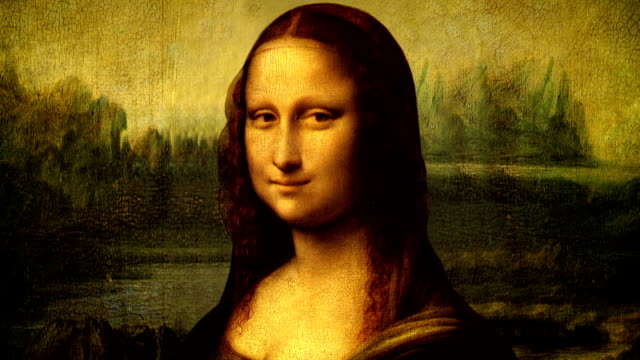
\includegraphics[width = 9cm]{portrait}}; 
%     % if necessary the picture may be moved by changing the at (coordinates)
%     % width defines the 'zoom' of the picture
% \end{tikzpicture}
% \hfill\vline\hfill
% \end{minipage}
% \begin{minipage}[c]{0.4\textwidth}
%     \textbf{\Huge \scshape{Ming Fang}} \\ \vspace{1pt} 
%     % \scshape sets small capital letters, remove if desired
%     \small{+1 217-305-1769} \\
%     \href{mailto:mingf2@illinois.edu}{\underline{mingf2@illinois.edu}}\\
%     % % Be sure to use a professional *personal* email address
%     % \href{https://www.linkedin.com/in/charles-rambo/}{\underline{linkedin.com/in/charles-rambo}} \\
%     % % you should adjust you linked in profile name to be professional and recognizable
%     % \href{https://github.com/fizixmastr}{\underline{github.com/fizixmastr}}
% \end{minipage}

% Without picture
\begin{center}
    \textbf{\Huge \scshape Ming Fang} \\ \vspace{1pt} %\scshape sets small capital letters, remove if desired
    \small 
    +1 217-305-1769 $|$
    \href{mailto:mingf2@illinois.edu}{{mingf2@illinois.edu}} $|$
    \href{{https://www.linkedin.com/in/ming-fang1}}{linkedin.com/in/ming-fang1}\\ \vspace{1pt}
    {1615 Melrose Park Ct, Apt 2022, Urbana, IL 61801, US}
    % {US ADD: 1615 Melrose Park Ct, Apt 2022, Urbana, IL 61801, USA}\\ \vspace{1pt}
    % {Foreign ADD: 9 Wazaoji Road, Yaoxitang Village, Mohuan Township, Longyou County, Quzhou, Zhejiang, China 324400}
    % % % Be sure to use a professional *personal* email address
    % \href{www.linkedin.com/in/ming-fang1}{\underline{linkedin.com/in/ming-fang1}} $|$
    % % you should adjust you linked in profile name to be professional and recognizable
    % \href{https://github.com/fizixmastr}{\underline{github.com/fizixmastr}}
\end{center}



\begin{comment}
This CV was written for specifically for positions I was applying for in
academia, and then modified to be a template.

A standard CV is about two pages long where as a resume in the US is one page.
sections can be added and removed here with this in mind. In my experience, 
education, and applicable work experience and skills are the most import things
to include on a resume. For a CV the Europass CV suggests the categories: Work
Experience, Education and Training, Language Skills, Digital Skills,
Communication and Interpersonal Skills, Conferences and Seminars, Creative Works
Driver's License, Hobbies and Interests, Honors and Awards, Management and
Leadership Skills, Networks and Memberships, Organizational Skills, Projects,
Publications, Recommendations, Social and Political Activities, Volunteering.

Your goal is to convey a who, what , when, where, why for every item you share. 
The who is obviously you, but I believe the rest should be done in that order.
For example below. An employer cares most about the degree held and typically 
less about the institution or where it is located (This is still good 
information though). Whatever order you choose be consistent throughout.
\end{comment}

% \section{Research Interest}
%   \CVItemListStart
%     \CVItem{Development of non-destructive assay methods of special material for the characterization of tri-structural isotropic particle (TRISO) fuel for pebble bed reactors.}
%     \CVItem{Development of single-volume scatter camera with SiPM scintillator readout.}
%     \CVItem{Radiation detector signal processing algorithms with a focus on accelerated Monte Carlo implementation and iterative linear inverse solver for image reconstruction.}
%     \CVItem{Application of advanced radiation detection techniques, such as positron lifetime spectroscopy.}
%   \CVItemListEnd
 
%-----EDUCATION----------------------------------------------------------------
\section{Education}
  \CVSubHeadingListStart
%    \CVSubheading % Example
%      {Degree Achieved}{Years of Study}
%      {Institution of Study}{Where it is located}
    \CVSubheading
      {{PhD Candidate $|$ \emph{\small{Nuclear, Plasma, and Radiological Engineering}}}}{Jan 2020 -- Present}
      {University of Illinois at Urbana-Champaign (UIUC)}{Urbana, USA}
      \CVItemListStart
        \CVItem{Cumulative GPA:  4.0 / 4.0}
      \CVItemListEnd
    \CVSubheading
      {{Master of Science $|$ \emph{\small{Nuclear, Plasma, and Radiological Engineering}}}}{Aug 2018 -- Dec 2019}
      {University of Illinois at Urbana-Champaign (UIUC)}{Urbana, USA}
       \CVItemListStart
        \CVItem{Cumulative GPA:  4.0 / 4.0}
      \CVItemListEnd
    \CVSubheading
      {{Bachelor of Engineering $|$ \emph{\small{Nuclear Engineering and Technology}}}}{Sept 2014 -- June 2018}
      {University of Science and Technology of China (USTC)}{Hefei, China}
       \CVItemListStart
        \CVItem{Cumulative GPA:  3.89 / 4.3}
      \CVItemListEnd
  \CVSubHeadingListEnd

%-----Research and projects----------------------------------------------------------
\begin{comment}
try to briefly explain what you did and why it is relevant to the position you
are seeking
\end{comment}
\begin{comment}
Ideally the title of the work should speak for what it is. However if you feel
like you should explain more about why the project is applicable to this job,
use item list as is shown in the work experience section.
\end{comment}

\section{Research Experience}
  \CVSubHeadingListStart
%    \CVSubheading %Example
%      {What you did}{When you worked there}
%      {Who you worked for}{Where they are located}
%      \CVItemListStart
%        \CVItem{Why it is important to this employer}
%      \CVItemListEnd
    \CVSubheading
      {Multi-Mode Imaging for TRISO-fueled Pebble Identification}{Aug 2020 - Present}
      {Graduate Research Assistant, Advisor: Prof. Angela Di Fulvio, UIUC}{Urbana, USA}
      \CVItemListStart
        \CVItem{Developed SCALE/MCNP models of advanced nuclear reactors and performed criticality/burnup calculation.}
        \CVItem{Designed a boron-coated straw-based neutron multiplicity counter in MNCP to perform non-destruction assay of fuel pebbles.}
        \CVItem{Implemented an accelerated Monte-Carlo algorithm in C++ to simulate X-ray images of a pebble generated by an industrial CT scanner.}
        \CVItem{Developed image reconstruction, image segmentation, and fuel pebble identification algorithms in python.}
        \CVItem{Contributed to the writing of the awarded Phase II STTR DOE grant.}
      \CVItemListEnd
    % \CVSubheading
    %   {Neutron and Compton Imager Design}{June 2020 - Present}
    %   {UIUC}{Urbana, USA}
    %   \CVItemListStart
    %     \CVItem{Designed a planar neutron imager using organic scintillators and implemented a back-projection algorithm to perform image reconstruction.}
    %     \CVItem{Designed a compact Compton imager using a CsI(Tl) scintillator and silicon photon multipliers (SiPM).}
    %     \CVItem{Created a printed circuit board for SiPM hosting and signal readout.}
    %   \CVItemListEnd
    \CVSubheading
      {Quantitative Image Reconstruction in Passive Gamma Emission Tomography (PGET)}{Aug 2019 -- Sept 2020}
      {Graduate Research Assistant, Advisor: Prof. Angela Di Fulvio, Prof. Yoann Altmann, UIUC}{Urbana, USA}
      \CVItemListStart
        \CVItem{Developed a linear forward model in C++ to characterize PGET system response to spent nuclear fuel assemblies in water cools.}
        \CVItem{Implemented an accelerated Monte Carlo algorithm in C++ to perform gamma-ray down-scattering correction.}
        \CVItem{Developed a full set of software in python to reconstruct cross-sectional images of inspected fuel assemblies, identify missing fuel pins, and estimate fuel pin activities.}
      \CVItemListEnd
    \CVSubheading
      {Active Interrogation Using a DD Neutron Generator}{May 2019 -- May 2020}
      {Graduate Research Assistant, Advisor: Prof. Angela Di Fulvio, UIUC}{Urbana, USA}
      \CVItemListStart
        \CVItem{Implemented a shift-register algorithm in python to calculate the coincidence neutron count rate.}
        \CVItem{Demonstrated the possibility of using a DD generator as a neutron active interrogation source based on the strong correlation between the time-dependent neutron count rate signature and uranium mass.}
      \CVItemListEnd
    \CVSubheading
      {Positron Annihilation Lifetime Spectroscopy (PALS)}{Jan 2019 – May 2019}
      {Graduate Research Assistant, Advisor: Prof. Angela Di Fulvio, UIUC}{Urbana, USA}
      \CVItemListStart
        \CVItem{Developed and optimized a PALS experimental setup using organic scintillators and fast digitizers.}
        \CVItem{Implemented an interpolation-based constant-fraction discrimination (CFD) timing algorithm in C++ to determine the pulse arrival time.}
      \CVItemListEnd
    % \newpage
    \CVSubheading
      {General-Purpose Pulse-Processing Program}{Sept 2018 – Present}
      {Graduate Research Assistant, Advisor: Prof. Angela Di Fulvio, UIUC}{Urbana, USA}
      \CVItemListStart
        \CVItem{Developed a fast and general-purpose pulse-processing program based on the CERN ROOT framework in C++.}
        \CVItem{Pulse-processing capabilities include zero suppression, pile-up rejection, pulse shape discrimination (PSD), CFD timing, coincidence selection, energy calibration, etc.}
        \CVItem{Visualization capabilities include waveform plot, pulse height distribution/pulse integral distribution plot, PSD plot, time-of-flight plot, etc.}
      \CVItemListEnd
    \CVSubheading
      {Implementation of Key Algorithms in Gamma Spectrum Analysis Software}{July 2017 – Mar 2018}
      {Undergraduate Research Assistant, Advisor: Dr. Jia Li, USTC}{Hefei, China}
      \CVItemListStart
        \CVItem{Implemented pulse smoothing, peak finding and background subtraction algorithms in C++.}
        \CVItem{Implemented energy calibration algorithm in C++.}
      \CVItemListEnd
  \CVSubHeadingListEnd

%-----PUBLICATIONS-------------------------------------------------------------
\section{Publications}

\hspace{1.5em}\textbf{Peer-Reviewed Journal Publications}
\begin{enumerate}
    % \item \bibentry{fang2021active}
    \item \bibentry{bcs2023}
    \item \bibentry{bcs2022}
    \item \bibentry{PGET20200706}
    \item \bibentry{eldaly2021bayesian}
    \item \bibentry{liu2021neutron}
    \item \bibentry{weiss2021effect}
    \item \bibentry{rebei2020quantitative}
    \item \bibentry{fang2019positron}
\end{enumerate}

\hspace{1.5em}\textbf{Proceedings at International Conferences}
\begin{enumerate}
% \setcounter{enumi}{0}
    \item \bibentry{MingNMCINMM2023}
    \item \bibentry{MingIEEENSS2022}
    \item \bibentry{Jacobieeenssmic2022}
    \item \bibentry{MingNMCINMM2022}
    \item \bibentry{MingTRISOANS2022}
    \item \bibentry{MingIEEENSS2021}
    \item \bibentry{ZhihuaINMM-ESARDA2021}
    \item \bibentry{WeissINMM-ESARDA2021}
    \item \bibentry{MingTRISOANSstudent2021}
    \item \bibentry{SatwikANSstudent2021}
    \item \bibentry{ZhihuaANSstudent2021}
    \item \bibentry{MingIEEENSS2020}
    \item \bibentry{fanginmm2020}
    \item \bibentry{fang2019timing}
    % \item \bibentry{Jonieeenssmic2022}
\end{enumerate}

%-----CONFERENCES AND PRESENTATIONS--------------------------------------------
\begin{comment}
Again the title should have already been enough, but if it is necessary to add
descriptions maintain the consistency from prior sections
\end{comment}
\section{Presentations at International Conferences}
    \begin{enumerate}
        \item \bibentry{NMCINMM2023}
        \item \bibentry{2022IEEENSSMIC}
        \item \bibentry{NMCINMM2022}
        \item \bibentry{TRISOANS2022}
        \item \bibentry{2021IEEENSSMIC}
        \item \bibentry{TRISOANS2021}
        \item \bibentry{2020IEEENSSMIC}
        \item \bibentry{2020INMM}
        \item \bibentry{2019IEEENSSMIC}
    \end{enumerate}
 
%-----TEACHING EXPERIENCE------------------------------------------------------
\begin{comment}
Section is here as it applied to my application for positions in academia. 
Remember to tailor the resume for to the position.
\end{comment}
% \section{Appointments}
% \CVSubHeadingListStart
% %    \CVSubheading %Example
% %      {What}{When}
% %      {Short Description}{}
%     \CVSubheading
%       {Graduate Research Assistant}{Sept 2018 – Present}
%       {Neutron Measurement Laboratory}{Urbana, USA}
%   \CVSubHeadingListEnd

\section{Teaching and Mentoring}
\CVSubHeadingListStart
    \CVSubheading
      {Seminars}{}
      {UIUC}{Urbana, USA}
      \CVItemListStart
        \CVItem{Course: NPRE451 NPRE Laboratory, Fall 2022}
        \CVItem{Course: NPRE452 Advanced Radiological Laboratory, Spring 2022, Fall 2022}
      \CVItemListEnd
    \CVSubheading
      {Outreach Activities}{Mar 2020}
      {UIUC}{Urbana, USA}
      \CVItemListStart
        \CVItem{Coordinated lab tour for the Academic Redshirt in Science and Engineering (ARISE).}
      \CVItemListEnd
    % \newpage
    \CVSubheading
      {Mentor}{Sept 2018 – Present}
      {UIUC}{Urbana, USA}
      \CVItemListStart
        \CVItem{Jacob Fritchie, Master student.}
        \CVItem{Satwik Pani, Undergraduate student.}
        \CVItem{Muzammil Siddiqui, Undergraduate student.}
        \CVItem{Noah Rebei, High School Summer Research Program, University Laboratory High School.}
      \CVItemListEnd
    \CVSubheading
      {Undergraduate Teaching Assistant}{Sept 2017 – Jan 2018}
      {USTC}{Hefei, China}
      \CVItemListStart
        \CVItem{Course: Physics, Subject: Quantum Mechanics B.}
      \CVItemListEnd
  \CVSubHeadingListEnd

%-----SKILLS-------------------------------------------------------------------
\begin{comment}
This section is compressed from the various skills sections that Euro CV
recommends.
\end{comment}

\section{Skills}
 \begin{itemize}[leftmargin=0.5cm, label={}]
    {\item{
     \textbf{Programming}{: C/C++, OpenMP/MPI, Python (NumPy, SciPy, Matplotlib), Bash, Java} \\
     \textbf{Document Creation}{: \LaTeX, Markdown, Microsoft Office Suite} \\
     \textbf{Software}{: MCNP, SCALE, MATLAB, Mathematica, ROOT, Git, CMake/Make, SOLIDWORKS, OrCAD Capture and PCB Editor, Origin, Vivado}\\
    }}
 \end{itemize}


%-----HONORS AND AWARDS--------------------------------------------------------
\section{Honors and Awards}
\CVSubHeadingListStart
    \CVSubheading
          {J.D. Williams Student Paper Award, Second Place}{July 2022}
          {Institute of Nuclear Materials Management 63rd Annual Meeting}{}
    \CVSubheading
          {ACDIS Summer 2022 Fellowship}{May 2022}
          {The Program in Arms Control \& Domestic and International Security (ACDIS), UIUC}{}
    \CVSubheading
          {Fellow of Exotic Beam Summer School}{June 2019}
          {Oak Ridge National Laboratory}{}
    \CVSubheading
          {Outstanding Teaching Assistant}{Mar 2018}
          {USTC}{}
    \CVSubheading
          {Outstanding Student Scholarship}{May 2017}
          {USTC}{}
    \CVSubheading
          {Institute of Modern Physics, Chinese Academy of Sciences Scholarship}{Sept. 2017}
          {USTC}{}
    \CVSubheading
          {Outstanding Student Scholarship}{May 2016}
          {USTC}{}
    \CVSubheading
          {Institute of Modern Physics, Chinese Academy of Sciences Scholarship}{Sept. 2015}
          {USTC}{}
    \CVSubheading
          {Outstanding Freshman Scholarship}{Sept. 2014}
          {USTC}{}
\CVSubHeadingListEnd

\section{Professional Societies}
\begin{itemize}
    \item Student member of Institute of Electrical and Electronics Engineers (IEEE)
    \item Student member of IEEE Nuclear and Plasma Sciences Society
    \item Secretary, Institute of Nuclear Materials Management UIUC Student Chapter
    \item Student member of Institute of Nuclear Materials Management
    \item Student member of American Nuclear Society
\end{itemize}
\end{document}